\chapter{Truth Studies}



\begin{figure}[h]
D  \centering
  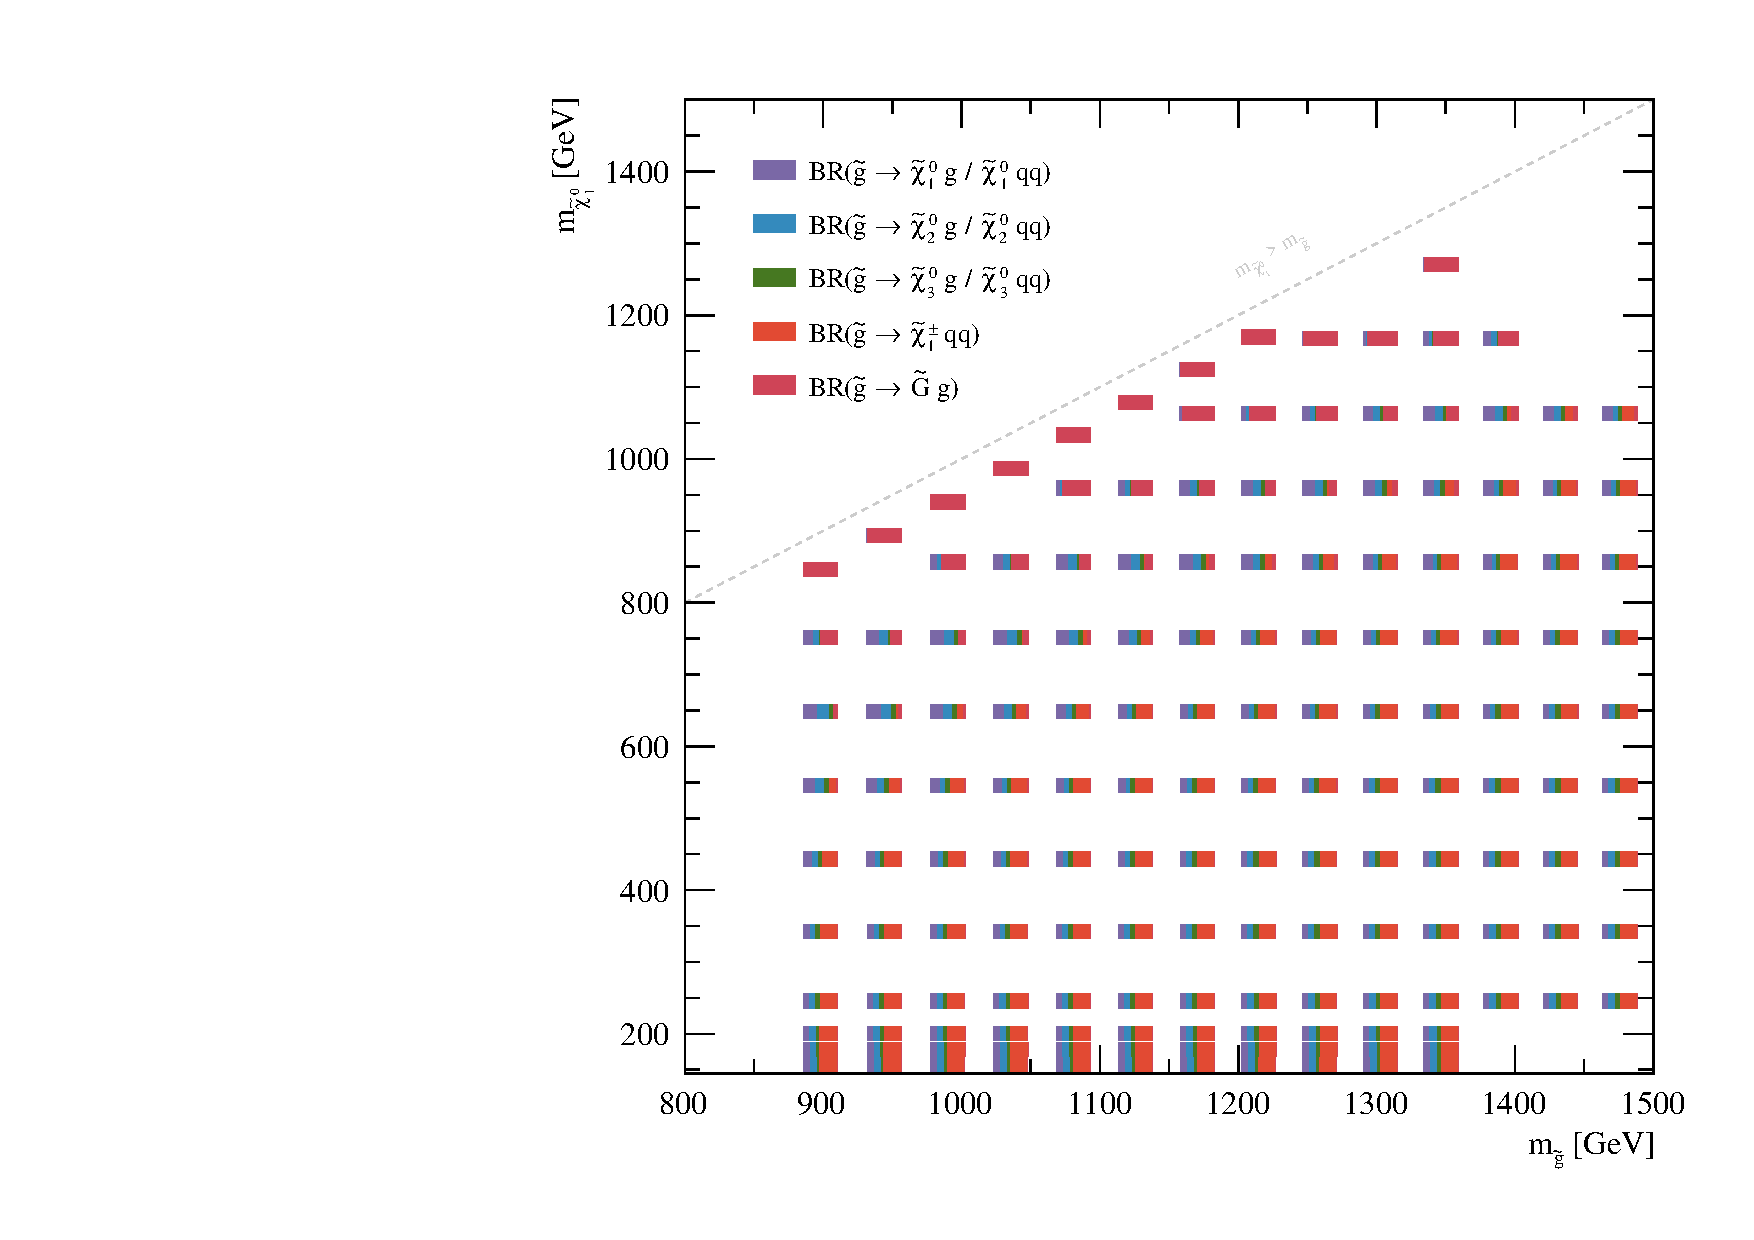
\includegraphics[width=0.8\textwidth]{figures/truth/br_gl_X}
  \caption{BR de los gluinos para los distintos puntos de la grid.}
\end{figure}

\begin{figure}[h]
  \centering
  \includegraphics[width=0.8\textwidth]{figures/truth/br_gl_2b_vs_3b}
  \caption{BR de los gluinos para los distintos puntos de la grid.}
\end{figure}

\begin{figure}[h]
  \includegraphics[width=0.8\textwidth]{figures/truth/br_gl_X_2body}
  \includegraphics[width=0.8\textwidth]{figures/truth/br_gl_X_3body}
 \caption{BR de los gluinos para los distintos puntos de la grid.}
\end{figure}


\begin{figure}[h]
  \centering
  \includegraphics[width=0.8\textwidth]{figures/truth/br_c1_X}
  \caption{BR de los gluinos para los distintos puntos de la grid.}
\end{figure}

\begin{figure}[h]
  \centering
  \includegraphics[width=0.8\textwidth]{figures/truth/br_n3_X}
  \caption{BR de los gluinos para los distintos puntos de la grid.}
\end{figure}

\begin{figure}[h]
  \centering
  \includegraphics[width=0.8\textwidth]{figures/truth/br_n2_X}
  \caption{BR de los gluinos para los distintos puntos de la grid.}
\end{figure}

\begin{figure}[h]
  \centering
  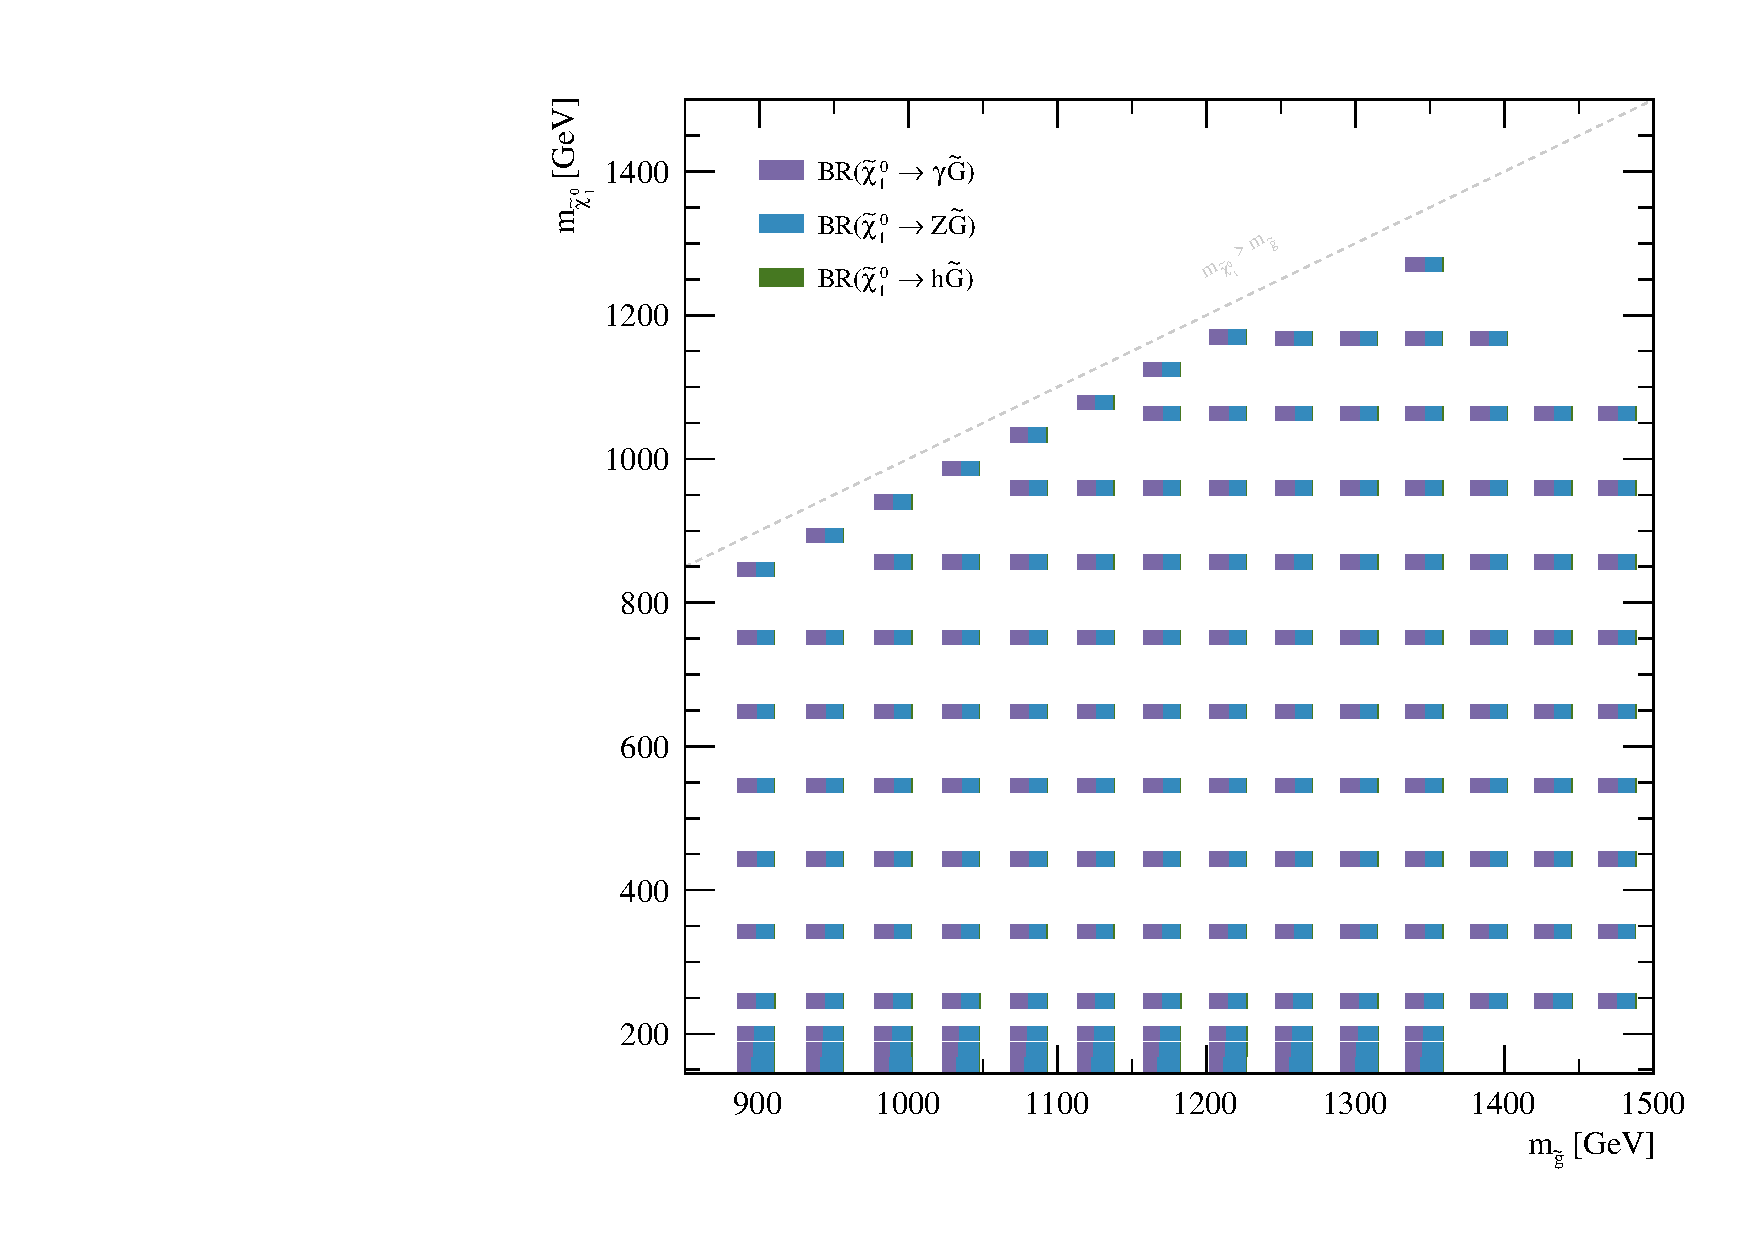
\includegraphics[width=0.8\textwidth]{figures/truth/br_n1_X}
  \caption{BR de los gluinos para los distintos puntos de la grid.}
\end{figure}
